\chapter{实验与分析}\label{chap:analysis}
%gshare,为了避免gshare的冷启动,而添加的一个仲裁策略。
%纸上读来终觉浅,觉知此事要躬行。前面梳理了很多乱序多发射设计的相关工作与材料,最终还需要能转化为自己的设计。不过在设计之前,必须有一套开发验证的方法和平台,和一套成型的循序渐进由易到难的设计方案。这两个要素是开始设计必备的前提条件。

\section{仿真实验平台}

本科学习期间采用的指令集是MIPS32,实验课上设计的单发射五级静态流水线处理器是基于龙芯提供的实验平台。设计中经历的步骤程序有:\textbf{step1}: 仿真时与龙芯提供的处理器loogson132生成(打印)的写回级trace对自动化的逐拍比对$ \Rightarrow $\textbf{step2}: 若比对出现不同则停止仿真,通过看波形找到产生不同写回信息的原因,并修正之$ \Rightarrow $如此循环往复直到仿真调通$ \Rightarrow $\textbf{step3}: 之后再用Vivado的集成化工具综合布局布线$ \Rightarrow $\textbf{step4}: 最后生成bitstream --- 可配置FPGA的格式文件,用JTAG线下载至Xilinx公司的FPGA上,产生物理上预期的效果就算设计完成。需要注意的是为了简化,课上实验中的内存是使用板卡上的SRAM模拟的,并不是真正的内存。

但是这样一套比较熟悉的平台,却很难将RISC-V移植进来。没有现成的可以用来比对的标准trace;Chisel代码内部逻辑变量没有很好的波形调试。所以原来的实验平台并不奏效。

很自然会想到在RISC-V开源处理器仓库中有没有可以略加修改便可使用的设计验证平台,于是尝试着阅读了Rocket和BOOM的说明文档及其代码。BOOM外围的很多代码是复用Rocket的,意味着存在着一种可能性 --- 区分出BOOM处理器自身和复用的Rocket代码,找到两者之间的接口,然后把BOOM替换为自主设计的处理器核心。但是不得不说,阅读代码的过程非常痛苦。首先BOOM和Rocket都是达到工业级别的颇为成熟的大工程了,里面的文件众多,每个文件中又有不同的类,这些类之间又有着非常复杂的交互关系。其次这些处理器的设计者和Chisel编译器的设计者属于一个团队,里面灵活使用了很多Chisel和Scala中高级的语言特性来更为简洁,扩展性更强的描述电路,但是这些特性却是初学者一时很难理解的障碍。加之本设计的任务并不是在BOOM的基础上添加模块,也不是修改BOOM的微结构来达到性能的提高(再者说,这样难免有抄袭之嫌),任务在于自主设计出一款和BOOM一样完整的处理器内核。所以如果需要和BOOM一样复用Rocket的外围代码,然后去跑仿真验证,就必须清楚的了解其中的没一个细节,这一个熟悉的过程最少也需要几个月的时间,时间上不允许。

最后采用的是加州大学伯克利分校体系结构课教学配套的适用于初学者的实验平台。如今,这个实验平台以及几个简单的能够在平台上运行的处理器核已经作为伯克利分校RISC-V开源仓库列表\href{https://github.com/ucb-bar/}{ucb-bar}中的\href{https://github.com/ucb-bar/riscv-sodor}{riscv-sodor仓库}开源了。另外,还有一个\href{https://gitter.im/librecores/riscv-sodor}{论坛社区}(\url{https://gitter.im/librecores/riscv-sodor})来答疑和解释该平台运行的机制。其机制可以简化地用图\ref{fig:platform}来概括。
\begin{figure}[!htbp]
	\centering
	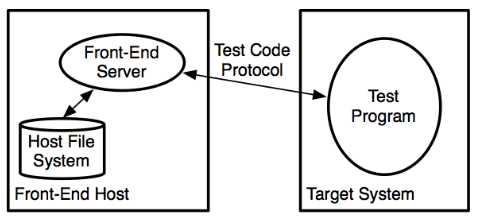
\includegraphics[width=0.5\linewidth]{platform}
	\bicaption{测试环境。前端服务器将RISC-V二进制文件加载到主机的文件系统中,启动目标系统的模拟器,发送RISC-V二进制代码到目标模拟器填充入模拟的处理器指令内存中。一旦前端服务器完成发送测试代码后,服务器重启目标处理器然后目标处理器就可以始从固定的地址开始执行程序。\citep{lab1}图2.}{The Testing Environment. The front-end server (fesvr) loads the RISC-V binary from the Host file system, starts the Target system simulator, and sends the RISC-V binary code to the Target simulator to populate the simulated processor’s instruction memory with the program. Once the fesvr finishes sending the test code, the fesvr resets the Target processor and the Target processor begins execution at a fixed address in the program. Figure 2 of \citep{lab1}.}
	\label{fig:platform}
\end{figure}

对这个实验平台,稍作修改,将原来糅杂在一起的处理器Chisel源代码,测试程序代码和测试工具链(如fesvr和生成C++模拟器的库文件)分离成两个相对独立的私有仓库,用git来管理,使得代码的编写工作变得更有条理。一级的文件目录结构如图\ref{fig:project}所示。另外,对原来处理器源码的组织形式做了略微的调整,使得更符合JAVA的代码组织结构风格。对于Makefile编译文件,也做了必要的修改,使之符合修改后的文件目录组织。
\begin{figure}[!htbp]
	\centering
	\begin{subfigure}[b]{0.4\textwidth}
		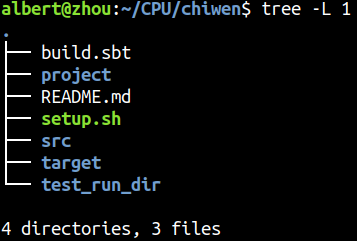
\includegraphics[width=\textwidth,height=4cm]{chiwen_L1}
		\caption{}
		\label{fig:chiwen_L1}
	\end{subfigure}\qquad%
	~%add desired spacing
	\begin{subfigure}[b]{0.4\textwidth}
		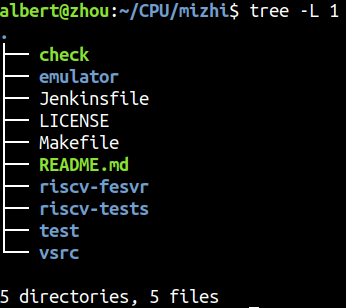
\includegraphics[width=\textwidth,height=4cm]{mizhi_L1}
		\caption{}
		\label{fig:mizhi_L1}
	\end{subfigure}
	\bicaption{毕业设计工程仓库。(a) 处理器Chisel源代码仓库。(b) 测试软件工具链和测试程序仓库。}{the repositories of the design. (a) The git repository which contains processors Chisel source, (b) The git repository which contains verification tool chain and test programs.}
	\label{fig:project}
\end{figure}

运行的流程大致为:
\begin{enumerate}[label=(\alph*)]
	\item 在\texttt{chiwen}目录下运行sbt,Scala的构建工具或者说是集成化的编译器(Chisel的编译器实际上是在sbt中加入前端的Chisel语法树分析,和后端的Chisel到Verilog的转化规则)。然后选择处理器的工程名,这样sbt就会产生一个处理器的C++精确到周期的描述。为了简化这一步骤,如图\ref{fig:chiwen_L1}编写了一个脚本,执行命令{\footnotesize \verb|terminal| -> \verb|./setup.sh <processor_name>|}即可。这个脚本最后会把生成的Verilog代码和Chisel的中间层表示Firrtl格式文件放到\texttt{mizhi}的\texttt{emulator}目录中以处理器命名的目录下。
	\item 编译文件Makefile会用verilator软件将第一步得到的生成代码再生成和处理器对应的C++模拟器。
	\item 编译文件Makefile会调用RISC-V的前端服务器(fesvr)在文件系统中为第二步得到的C++二进制模拟器打开一个socket,然后将RISC-V的二进制文件文件传输到目标处理器去执行,见图\ref{fig:platform}.
	\item 在\texttt{mizhi}仓库里,已经提供了现成的测试程序包括指令功能测试和嵌入式benchmark程序性能测试,其中的benchmark程序集如表\ref{tab:benchmark}所示。所有测试程序位于\texttt{riscv- tests}目录中;自定义的测试程序,可以放至test目录中,见图\ref{fig:mizhi_L1}。 程序的编译用RV32I的GCC工具链标准编译。具体的命令封装在Makefile中,只需要输入命令{\footnotesize \verb|cd riscv-tests/isa| -> \verb|make|}生成指令测试二进制文件或者{\footnotesize \verb|cd riscv-tests/benchmarks| -> \verb|make|}生成性能测试的二进制文件。相应的,让目标处理器去仿真模拟执行只需要输入命令{\footnotesize \verb|make run-asm-tests|}或者{\footnotesize \verb|make run-bmarks-test|}就能运行指令功能测试或者benchmark性能测试。
	\item 最后如果通过,会在终端给出PASSED字样,否则就是FAILED来给出处理器的验证结果。大致的机理是Makefile会先用Spike,RISC-V的ISA级模拟器跑出一遍trace,然后比对处理器的输出结果。前端服务器(fesvr)也会通过debugIO通过访存来检测处理器的状态是否达到预期。不过存在着自动检测在FAILED时却给出PASSED的少见情况。针对这种情况,用python编写了一个脚本来比对待测试处理器产生的trace和Spike跑出的标准trace每一个周期的有效写回寄存器堆结果,或者也可以和sodor已经提供的几个简单处理器打印的trace做对比。这样就能严格保证处理器执行已有程序的正确性。
\end{enumerate}

\section{设计方案}
\begin{figure}[H]
	\centering
	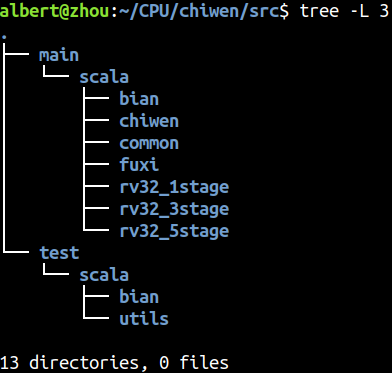
\includegraphics[width=0.4\linewidth]{chiwen_src_L3}
	\bicaption{目前为止已有的六款RISC-V RV32I处理器核。其中3款处理器CHIWEN(螭吻), FUXI, BIAN(狴犴)架构分别是自主设计的单发射五级静态流水线,双发射五级静态流水线, 和双发射乱序流水线。另外3款rv32\_1stage, rv32\_3stage, rv32\_5stage是\href{https://github.com/ucb-bar/riscv-sodor}{riscv-sodor}提供的单周期、单发射三级静态流水线和单发射五级静态流水线处理器。common子目录包含了处理器共有的模块。}{The six Microprocessors based on RISC-V RV32I isa so far. There are three processors are self designed, including CHIWEN(single-issue, five-stage pipeline processor), FUXI(dual-isse, five-stage pipeline processor) and BIAN(two-wide superscalar processor with out-of-order). Other three simple processors are provided by \href{https://github.com/ucb-bar/riscv-sodor}{riscv-sodor}, with single cycle, three-stage and five stage single-issue architecture separately. \texttt{common} subdirectory contains common modules shared with all processors.}
	\label{fig:chiwen_src}
\end{figure}

若直接进行双发射乱序的设计,会因为没有很好的设计着力点而变得步履维艰。所以制定出一套详细的从易到难循序渐进的方案显得非常重要。同时,Chisel对于自己来说是一门全新的语言,也需要用一些简单的任务来充分地熟悉。

在riscv-sodor中已经提供的有三款简单的处理器,微结构分别是单周期(rv32\_1stage)、单发射三级静态流水线(rv32\_1stage)和单发射五级静态流水线(rv32\_5stage)。将它们拷贝至自己的仓库的文代码目录中,参见图\ref{fig:chiwen_src}。这些简单的处理器除去共有的CSR特权寄存器逻辑和仿真内存逻辑代码之外,核心部分均仅仅只有500多行代码,代码简洁易读,尤其是其译码部分。处理器采用的结构是经典的数据通路和指令通路。但是事实上这样的设计模式不好,两个通路之间是强耦合的。在阅读rv32\_5stage的过程中,也发现数据通路和控制通路的两个文件中相当有一部分代码重复冗余。为了可拓展性和控制复杂性的考虑,第一步是调整处理器的设计模式,采用章节\ref{sec:model}中论及的前后端模型。修改的同时,逐渐掌握了Chisel描述电路的常用写法。

\begin{table}[!htbp]
	\bicaption{benchmark性能测试程序说明。除了coremark是自己添加的,其余的都是\href{https://github.com/riscv/riscv-tests}{riscv-tests}已经提供的}{The explanation of the set of benchmarks provided by the  \href{https://github.com/riscv/riscv-tests}{riscv-tests} repository except for coremark}
	\label{tab:benchmark}
	\centering
	\footnotesize% fontsize
	\setlength{\tabcolsep}{4pt}% column separation
	\renewcommand{\arraystretch}{1.2}%row space 
	\begin{tabular}{lcc}
		\hline
		名称 & 功能解释 & 备注 \\%inserts table 
		%\cline{2-9}% partial hline from column i to column j
		\hline
		coremark    & A synthetic embedded integer benchmark      & 合成的嵌入式整数程序 \\
		dhrystone   & A synthetic embedded integer benchmark.     & 合成的嵌入式整数程序 \\
		median 		& Performs a 1D three element median filter.  & 一维的中位数查找 \\
		multiply 	& A software implementation of multiply.      & 乘法的软件实现 \\
		qsort  		& Sorts an array of integers using quick sort. & 快速排序 \\
		rsort  		& Sorts an array of integers using radix sort. & 基数排序 \\
		towers 		& Solves the Towers of Hanoi puzzle recursively. & 汉诺塔 \\
		vvadd 		& Sums two arrays and writes into a third array. & 数组向量加法 \\
		\hline
	\end{tabular}
\end{table}

但是CHIWEN不是对rv32\_5stage简单重写。事实上,rv32\_5stage运行benchmark的统计结果如图\ref{fig:rv32_sodor}所示,IPC普遍偏低。
\begin{figure}[!htbp]
	\begin{tikzpicture}
	\begin{axis}[
	width=0.85*\textwidth,
	height = 8cm,
	ybar=2*\pgflinewidth,
	bar width=14pt,
	ylabel = {Instruction per Cycle},
	ymajorgrids = true,
	xtick=data,
	x tick label style={rotate=-45, anchor=west},
	symbolic x coords={coremark,dhrystone,median,multiply,qsort,rsort,towers,vvadd},
	scaled y ticks = false,
	%enlarge x limits=0.25,
	ymin=0.4,
	]
	
	\addplot[style={ppurple,fill=ppurple,mark=none}]
	coordinates {(coremark, 0.69) (dhrystone,0.75) (median,0.69) (multiply,0.64) (qsort,0.64) (rsort,0.92) (towers,0.82) (vvadd,0.76)};
	
	\end{axis}
	\end{tikzpicture}
	\bicaption{rv32\_5stage运行benchmark程序集的IPC。}{the IPC of rv32\_5stage executing benchmark programs.}
	\label{fig:rv32_sodor}		
\end{figure}

导致性能偏低的原因在于rv32\_5stage没有转移猜测的机制,如果跳转指令的结果还没计算出来,只会顺序往后取指。RISC-V没有延迟槽,而且在rv32\_5stage的设计中,第三级计算出跳转目标和方向还会锁存一个周期反馈到取指部件进行重定向取指。所以猜错一个分支跳转指令就会损失2个周期,这样IPC就不会高。所以第二个任务就是在CHIWEN的前端加入转移预测器,参考借鉴的是文献\citet{Celio:EECS-2017-157}中的BTB,BPD和RAS设计,并做了一定简化。

在riscv-sodor平台上取指和访存都是没有延迟的,默认是同步的逻辑。为了模拟真实的外围内存系统,写了一个带有随机性的延迟的中间桥,置于处理器核和模拟的同步内存之间,并且采用的是AXI的标准接口。接着构建了容量为16KB的icache来缓存指令,提高在有延迟的取指环境中的处理器性能。但是出于简化设计的考虑,并没有构建dcache,访存没有延迟,为默认的同步时序。综上,基于前后端模型的五级流水线架构,辅以转移预测器和icache构成了CHIWEN处理器。

得益于前后端模式的强大优势,从单发射的CHIWEN过渡到超标量宽度为2的双发射五级静态流水线FUXI的过程非常平稳,代码基本上能够复用,不用做大的修改,开发的时间和调试的时间都大大缩短了。大致的修改如下:
\begin{enumerate}[label=(\alph*)]
	\item 后端的修改较为简单,把CHIWEN的后端用Chisel里Vec的写法重新写一遍,构建出两条并行的后端执行流水线。然后解决两条并行指令之间的如写后写、写后读、同时为跳转指令、同时为访存指令、同时为特权态指令等冲突。具体的解决做法是:将后一条指令停住一个周期做成串行执行。不光写起来简单,调试的时候也不会出现很多的bug。
	\item 前端的修改是重点,也是难点,修改取指单元,参见章节\ref{subsec:fetchi}。同时,icache和分支预测单元都要做出修改,将输入PC信号(if/pc级)和输出指令信号(icache)或预测信号(分支预测单元)从单端口调整为双端口。
\end{enumerate}

有了CHIWEN和FUXI这两代处理器核微结构的演进,才过渡到双发射乱序处理器BIAN的设计调试中。由于FUXI和BIAN都是超标量宽度为2的处理器,所以BIAN的前端可以完全复用FUXI的,而不需要单独重新设计。解决了前端的问题,最后只需集中力量进行后端乱序发射的逻辑设计即可。前后端强大的优势再次得到了很好的体现。而且可以看出,高性能双发射乱序处理器的成功设计离不开循序渐进的正确设计路线。

\section{调试手段}

首先是模块级的调试验证。Verilog常用的做法是给待测模块写激励测试。这个激励测试相当于更大一级的测试激励模块,里面实例化了待测模块并构建有时钟时序和测试输入,然后通过仿真器手动查看输出信号波形是否符合预期。缺点在于,激励模块的编写过程十分麻烦,不仅是因为语句的粒度太小描述能力差,而且入如果波形出现和预期不同的结果,也不能马上得出待测模块有漏洞的结论,因为也有可能是激励模块有漏洞。因此,Chisel语言自封闭的设计了一套基于Chisel和Scala编写验证模块的方式。它封装了\texttt{\footnotesize{chisel3.iotesters.PeekPokeTester}}的基类,编写待测模块的激励模块首先要继承这个基类,待测模块输入端的赋值调用poke语句,输出端的验证可以用expect语句和预期值进行自动比对,也可以打印出来。同时,因为Scala是脚本语言,所以复杂的且带随机性的激励测试构造是便捷的。另外,最为关键的一点是,\texttt{\footnotesize{chisel3.iotesters.PeekPokeTester}}基类隐藏了时序的构造,因为电路的何时复位,时钟的频率多少,何时在上升沿一般情况下不会对处理器电路产生任何影响。电路经过一个时钟周期的逻辑在Chisel的测试代码中可以用简单的\texttt{step(1)}实现(括号中的1表示一个周期)。语义上,在\texttt{step(1)}之后的代码逻辑会发生在\texttt{step(1)}之前的代码逻辑一个周期之后。Chisel的测试代码的组织形式和JAVA保持一致,见图\ref{fig:chiwen_src}中的test目录,这样方便管理和测试,特别是在IDE的编辑环境中。

但是上述调试方法不再适用于将各个模块整合起来的整个系统。整个系统的激励输入还是要依赖于riscv-sodor的测试环境(见图\ref{fig:platform})。那么输出端又如何去验证呢?输出端核心的信号有哪些?最核心的是每一周期的寄存器堆写回信号和store指令的内存写回信息。如果这两类信号都符合预期,就认为处理器的输出是正确的。这个预期可以由RISC-V的模拟器Spike或者QEMU得到,也可以由经过验证的开源处理器核如rv32\_5stage得到。调试的流程为:\textbf{step1}: 写回信息打印出来以文本的形式存储$ \Rightarrow $\textbf{step2}: 用自己编写的一个自动对比的python脚本进行文本操作自动比对$ \Rightarrow $\textbf{step3}: 定位到开始出现不同的第一个周期$ \Rightarrow $\textbf{step4}: 在源代码中加入在这个周期之前一个窗口内打印与产生差错有关联的更多变量的代码$ \Rightarrow $\textbf{step5}: 重新编译执行$ \Rightarrow $\textbf{step6}: 通过分析文本中的调试信息来定位到源代码中的bug。

这样调试方式虽然原始,如果需要重新加入打印信号,就需要重新编译执行。但是就其速度而言,因为不用做整个系统全信号的仿真模拟,仅仅是打印出是每一周期的写回信息以及一段窗口内的详细的相关变量信号而已,就算加上重新编译和执行的时间,也比波形图仿真更快。另外,由于设计的时候先采用了较为彻底的模块级验证,等到整合为完整系统时,bug数量大大降低了,而且基本集中在各个模块交互的逻辑上。同时,文本的优势在于可以灵活地编写一些文本操作的脚本做自动化的分析,这恰恰是波形所不具备的。比如需要得到某一周期执行级具体的指令,波形图上只能显示一个32位的数值,转化需要人工手动。但是文本就可以用一个脚本来自动转化。还有例如分析分支跳转预测正确率的过程中需要统计精确到不同跳转指令的误预测率时或者某一周期窗口内的跳转行为以及预测行为时,文本+脚本分析的手段都要明显优于波形图调试。

正是采用了这种调试手段,从最开始的调试方式摸索阶段,用两周时间调通了带转移预测器的CHIWEN处理器,并且预测器的行为符合预期;再到用一周时间调通FUXI的前端,加上三天调通FUXI的后端;最后到用两周的时间(一周进行模块级的调试验证,一周进行整合系统的调试验证)调通了整合到FUXI前端的BIAN的后端。调试的时间的缩短使得在微结构设计上的时间变得相对充裕。

\section{结果分析}
表\ref{tab:inst_number}是各个程序的大致动态指令数,以及运行的时候执行的指令数。之所以是大致,是因为由于一些与串口打印交互的轮循和依赖执行周期的汇编代码的存在,不同的处理器执行各个程序的行为会出现偏差,指令数也就不一样。可以看出coremark, dhrystone, qsort和rsort的规模比较大,达到了十万量级;而median, multiply, towers, vvadd的规模较小,为万量级。
\begin{table}[!htbp]
	\bicaption{benchmark各个程序大致动态指令数。}{The approximate number of dynamic instructions of each program in the benchmark.}
	\label{tab:inst_number}
	\centering
	\footnotesize% fontsize
	\setlength{\tabcolsep}{4pt}% column separation
	\renewcommand{\arraystretch}{1.2}%row space 
	\begin{tabular}{cc}
		\hline
		benchmark & 指令数 \\%inserts table 
		%\cline{2-9}% partial hline from column i to column j
		\hline
		coremark    & $ \sim $780K\\
		dhrystone   & $ \sim $350K\\
		median 		& $ \sim $15K\\
		multiply 	& $ \sim $49K\\
		qsort  		& $ \sim $230K\\
		rsort  		& $ \sim $370K\\
		towers 		& $ \sim $18K\\
		vvadd 		& $ \sim $11K\\
		\hline
	\end{tabular}
\end{table}

\begin{figure}[!htbp]
	\centering
	\begin{tikzpicture}
	[
	pie chart,
	slice type={arithmetic}{blu},
	slice type={branch}{rosso},
	slice type={load}{giallo},
	slice type={store}{viola},
	slice type={jal}{verde},
	slice type={jalr}{pink},
	pie values/.style={font={\small}},
	scale=2
	]
	
	\pie{coremark}
	{58.4/arithmetic,1.7/jalr,2.6/store,27.6/branch,1.8/jal,7.9/load}%
	\pie[xshift=2.2cm,values of coltello/.style={pos=1.1}]{dhrystone}
	{40.8/arithmetic,18.8/branch,19.0/load,12.2/store,3.7/jal,3.3/jalr}%
	
	\pie[yshift=-2.5cm,values of caffe/.style={pos=1.1}]{median}
	{32.5/arithmetic,30.8/branch,1.3/jalr,23.3/load,7.3/store,4.5/jal}%
	\pie[yshift=-2.5cm,xshift=2.2cm,values of caffe/.style={pos=1.1}]{qsort}
	{38.6/arithmetic,26.9/branch,24.0/load,7.3/store,3.1/jal}%
	\pie[yshift=-2.5cm,xshift=4.4cm,values of caffe/.style={pos=1.1}]{multiply}
	{64.4/arithmetic,0.9/jal,0.9/jalr,1.2/store,30.3/branch,2.3/load}%
	
	\pie[yshift=-5cm,values of caffe/.style={pos=1.1}]{rsort}
	{59.7/arithmetic,5.3/branch,20.4/load,14.4/store}%
	\pie[yshift=-5cm,xshift=2.2cm,values of caffe/.style={pos=1.1}]{towers}
	{43.0/arithmetic,2.8/jal,21.1/load,20.6/store,2.5/jalr,9.6/branch}%
	\pie[yshift=-5cm,xshift=4.4cm,values of caffe/.style={pos=1.1}]{vvadd}
	{48.6/arithmetic,1.7/jal,19.4/branch,1.8/jalr,19.9/load,8.4/store}%
	
	\legend[shift={(4cm,1cm)}]{{Arithmetic}/arithmetic,{Branch}/branch, {Load}/load}
	\legend[shift={(5cm,1cm)}]{{Store}/store,{Jal}/jal, {Jalr}/jalr}
	\end{tikzpicture}
	\bicaption{benchmark中各个程序不同指令的占比。Arithmetic: 算数指令;Branch: 分支指令; Load: 加载指令;Store: 存储指令;Jal: 立即数为偏移量的跳转链接指令;Jalr: 寄存器为偏移量的跳转链接指令。}{The ratios of different instruction types in every programs among the benchmark.}
	\label{fig:inst_types}
\end{figure}

图\ref{fig:inst_types}分析了八个程序不同类型指令的占比情况。可以看出,coremark, median, qsort, multiply四个程序分支跳转指令(Branch+Jal+Jalr)占比很大,均在30\%以上,相当于3条指令中就有一条分支跳针指令,非常密集。而dhrystone, rsort, towers, vvadd这四个程序转移跳转指令占比较为合理,属于一般意义上的正常程序。

\begin{figure}[!htbp]
	\centering
	\begin{tikzpicture}
	\begin{axis}[
		width=0.85*\textwidth,
		height = 10cm,
		ybar=2*\pgflinewidth,
		bar width=8pt,
		ylabel = {Instruction per Cycle},
		ymajorgrids = true,
		xtick=data,
		x tick label style={rotate=-45, anchor=west},
		symbolic x coords={coremark,dhrystone,median,multiply,qsort,rsort,towers,vvadd},
		scaled y ticks = false,
		%enlarge x limits=0.25,
		ymin=0.4,
		%legend pos=north west,
		legend style={at={(0.5,-0.20)},
		anchor=north,legend columns=-1}
	]
	
	\addplot[style={ggreen,fill=ggreen,mark=none}]
	coordinates {(coremark, 0.860) (dhrystone,0.946) (median,0.829) (multiply,0.913) (qsort,0.780) (rsort,0.993) (towers,0.884) (vvadd,0.853)};
	
	\addplot[style={bblue,fill=bblue,mark=none}]
	coordinates {(coremark, 1.122) (dhrystone,1.143) (median,0.982) (multiply,1.331) (qsort,0.866) (rsort,1.338) (towers,1.097) (vvadd,1.078)};
	
	\addplot[style={rred,fill=rred,mark=none}]
	coordinates {(coremark, 1.048) (dhrystone,1.269) (median,0.842) (multiply,1.254) (qsort,0.969) (rsort,1.553) (towers,0.981) (vvadd,1.119)};
	
	\legend{CHIWEN, FUXI, BIAN}
	\end{axis}
	\end{tikzpicture}
	\bicaption{三款处理器执行各个程序的每周期指令数。}{the Instruction per Cycle of each program over three processors.}
	\label{fig:ipc_result}
\end{figure}

如图\ref{fig:ipc_result},对比了3款处理器执行程序的性能(用IPC来衡量)。可以看到,最终结果并没有像预期一样,乱序双发射的BIAN执行各个程序都完美地优于顺序流水线架构下的CHIWEN和FUXI。BIAN对比单发射的CHIWEN,性能都是有所提高的。但是对比FUXI,却是互有胜负。dhystrone, qsort, rsort, vvadd处理器BIAN效率更高,而coremark, median, multiply, towers却是双发射顺序流水线的FUXI效率更高。

分析原因,首先非常直观的一个观察是在BIAN劣于FUXI的4个程序中,跳转分支指令占比大于30\%的占了3席:coremark, median, multiply. 为了更为客观的观察分支跳转指令对处理器性能的影响,图\ref{fig:accurate_result}专门统计了3款处理器运行各个程序的转移预测正确率,BIAN的预测正确率在82\%以下的一共有4个程序:coremark, median, qsort, towers. 其中,和BIAN性能劣于FUXI的4个程序重合了3个。coremard和median更是跌到80\%以下。所以coremark和median在没有访存延迟的环境下,乱序结构不如顺序结构性能高的现象基本上可以归因于转移跳转指令占比高的同时转移预测正确率又很低。

\begin{table}[!htbp]
	\bicaption{三款处理器执行各个程序的每周期指令数。}{the Instruction per Cycle of each program over three processors.}
	\label{tab:ipc_result}
	\centering
	\footnotesize% fontsize
	\setlength{\tabcolsep}{4pt}% column separation
	\renewcommand{\arraystretch}{1.2}%row space 
	\begin{tabular}{cccc}
		\hline
		benchmark & CHIWEN & FUXI & BIAN \\%inserts table 
		%\cline{2-9}% partial hline from column i to column j
		\hline
		coremark    & 0.860 & 1.122 & 1.048\\
		dhrystone   & 0.946 & 1.143 & 1.269\\
		median 		& 0.829 & 0.982 & 0.842\\
		multiply 	& 0.913 & 1.331 & 1.254\\
		qsort  		& 0.780 & 0.866 & 0.969\\
		rsort  		& 0.993 & 1.338 & 1.553\\
		towers 		& 0.884 & 1.097 & 0.981\\
		vvadd 		& 0.853 & 1.078 & 1.119\\
		\hline
	\end{tabular}
\end{table}

\begin{figure}[!htbp]
	\centering
	\begin{tikzpicture}
	\begin{axis}[
	width=0.85*\textwidth,
	height = 10cm,
	percentage plot,
	ybar=2*\pgflinewidth,
	bar width=8pt,
	ylabel = {Branch Prediction Accuracy},
	ymajorgrids = true,
	xtick=data,
	x tick label style={rotate=-45, anchor=west},
	symbolic x coords={coremark,dhrystone,median,multiply,qsort,rsort,towers,vvadd},
	scaled y ticks = false,
	%enlarge x limits=0.25,
	ymin=70,
	%legend pos=north west,
	legend style={at={(0.5,-0.20)},
		anchor=north,legend columns=-1}
	]
	
	\addplot[style={ggreen,fill=ggreen,mark=none}]
	coordinates {(coremark, 79.7) (dhrystone,94.6) (median,82.9) (multiply,89.1) (qsort,83.4) (rsort,97.3) (towers,82.4) (vvadd,87.2)};
	
	\addplot[style={bblue,fill=bblue,mark=none}]
	coordinates {(coremark, 80.0) (dhrystone,95.9) (median,80.6) (multiply,90.0) (qsort,83.4) (rsort,97.0) (towers,82.1) (vvadd,86.9)};
	
	\addplot[style={rred,fill=rred,mark=none}]
	coordinates {(coremark, 77.7) (dhrystone,93.7) (median,79.1) (multiply,90.0) (qsort,81.8) (rsort,97.8) (towers,81.7) (vvadd,89.0)};
	
	\legend{CHIWEN, FUXI, BIAN}
	\end{axis}
	\end{tikzpicture}
	\bicaption{三款处理器执行各个程序的转移预测正确率。}{The Branch Prediction Accuracy of each program over three processors.}
	\label{fig:accurate_result}
\end{figure}


\begin{table}[!htbp]
	\bicaption{三款处理器执行各个程序的转移预测正确率。}{The Branch Prediction Accuracy of each program over three processors.}
	\label{tab:accurate_result}
	\centering
	\footnotesize% fontsize
	\setlength{\tabcolsep}{4pt}% column separation
	\renewcommand{\arraystretch}{1.2}%row space 
	\begin{tabular}{cccc}
		\hline
		benchmark & CHIWEN & FUXI & BIAN \\%inserts table 
		%\cline{2-9}% partial hline from column i to column j
		\hline
		coremark    & 79.7\% & 80.0\% & 77.7\% \\
		dhrystone   & 94.6\% & 95.9\% & 93.7\% \\
		median 		& 82.9\% & 80.6\% & 79.1\% \\
		multiply 	& 89.1\% & 90.0\% & 90.0\% \\
		qsort  		& 83.4\% & 83.4\% & 81.8\% \\
		rsort  		& 97.3\% & 97.0\% & 97.8\% \\
		towers 		& 82.4\% & 82.1\% & 81.7\% \\
		vvadd 		& 87.2\% & 86.9\% & 89.0\% \\
		\hline
	\end{tabular}
\end{table}

从图\ref{fig:accurate_result}中还有一个有趣的现象是不同处理器执行同一程序的转移预测率是不同的。但是这三款处理器均是采用相同的数据结构和预测策略。产生这种现象的原因在于由于在流水线上,转移预测的数据结构的更新有反馈周期(解释见\ref{subsec:bj_unit})的延迟,不同微结构的反馈周期不同,有些预测的结果就是预测单元在结构未做更新时产生的,所以会对预测结果产生小范围的波动效应。

\begin{figure}[!htbp]
	\centering
	\begin{tikzpicture}[
	every axis/.style={ % add these settings to all the axis environments in the tikzpicture
		width=0.85*\textwidth,
		ylabel = {Instruction per Cycle},
		ybar stacked,
		ymin=0.7, ymax=1.6,
		x tick label style={rotate=-45, anchor=west},
		symbolic x coords={coremark,dhrystone,median,multiply,qsort,rsort,towers,vvadd},
		bar width=8pt,
		%legend style={at={(0.5,-0.20)},
		%anchor=north,legend columns=-1}
	},
	]
	% bar shift -10pt here chiwen
	\begin{axis}[bar shift=-10pt,hide axis,legend style={at={(0.36,-0.15)},
		anchor=north,legend columns=-1}]
	\addplot[style={ggreen,fill=ggreen,mark=none}]
	coordinates {(coremark, 0.856) (dhrystone,0.909) (median,0.781) (multiply,0.908) (qsort,0.779) (rsort,0.992) (towers,0.864) (vvadd,0.838)};
	%856 909 781 908 779 992 864 838
	\addplot[gray,fill=gray]coordinates
	{(coremark, 0.004) (dhrystone,0.037) (median,0.048) (multiply,0.005) (qsort,0.001) (rsort,0.001) (towers,0.020) (vvadd,0.015)};
	\legend{CHIWEN}
	\end{axis}
	
	zero bar shift here fuxi
	\begin{axis}[hide axis,legend style={at={(0.53,-0.15)},
		anchor=north,legend columns=-1}]
	\addplot+[style={bblue,fill=bblue,mark=none}]
	coordinates {(coremark, 1.110) (dhrystone,1.083) (median,0.927) (multiply,1.321) (qsort,0.864) (rsort,1.337) (towers,1.065) (vvadd,1.053)};
	%1.110 1.083 927 1.321 0.864 1.337 1.065 1.053
	\addplot+[gray,fill=gray]coordinates 
	{(coremark, 0.012) (dhrystone,0.06) (median,0.055) (multiply,0.01) (qsort,0.002) (rsort,0.001) (towers,0.032) (vvadd,0.025)};
	\legend{FUXI}
	\end{axis}
	
	% and bar shift +10pt here bian
	\begin{axis}[bar shift=10pt,legend style={at={(0.67,-0.15)},
		anchor=north,legend columns=-1}]
	\addplot+[style={rred,fill=rred,mark=none}]
	coordinates {(coremark, 1.051) (dhrystone,1.174) (median,0.773) (multiply,1.242) (qsort,0.975) (rsort,1.548) (towers,0.938) (vvadd,1.088)};
	%051 174 773 242 975 548 0.938 088
	\addplot+[gray,fill=gray]
	coordinates {(coremark, 0) (dhrystone,0.095) (median,0.069) (multiply,0.012) (qsort,0) (rsort,0.005) (towers,0.043) (vvadd,0.031)};
	%coremark qsort -
	\legend{BIAN}
	\end{axis}
	\end{tikzpicture}
	\bicaption{三款处理器只采用两位饱和计数器的BTB表预测技术,执行各个程序的每周期指令数。灰色部分是相比用原先预测策略的减少量。}{the instruction per cycle of each program for three processors which only use 2-bit BTB structure. The gray is the decrement compared with the original prediction strategy.}
	\label{fig:ipc_result_ruo}
\end{figure}



\begin{table}[!htbp]
	\bicaption{三款处理器只采用两位饱和计数器的BTB表预测技术,执行各个程序的每周期指令数。}{the instruction per cycle of each program for three processors which only use 2-bit BTB structure.}
	\label{tab:ipc_result_ruo}
	\centering
	\footnotesize% fontsize
	\setlength{\tabcolsep}{4pt}% column separation
	\renewcommand{\arraystretch}{1.2}%row space 
	\begin{tabular}{cccc}
		\hline
		benchmark & CHIWEN & FUXI & BIAN \\%inserts table 
		%\cline{2-9}% partial hline from column i to column j
		\hline
		coremark    & 0.856 & 1.110 & 1.051 \\
		dhrystone   & 0.909 & 1.083 & 1.174 \\
		median 		& 0.781 & 0.927 & 0.773 \\
		multiply 	& 0.908 & 1.321 & 1.242 \\
		qsort  		& 0.779 & 0.864 & 0.975 \\
		rsort  		& 0.992 & 1.337 & 1.548 \\
		towers 		& 0.864 & 1.065 & 0.938 \\
		vvadd 		& 0.838 & 1.053 & 1.088 \\
		\hline
	\end{tabular}
\end{table}

\begin{figure}[!htbp]
	\centering
	\begin{tikzpicture}[
	every axis/.style={ % add these settings to all the axis environments in the tikzpicture
		width=0.85*\textwidth,
		height=10cm,
		percentage plot,
		ylabel = {Branch Prediction Accuracy},
		ybar stacked,
		ymin=65,ymax=100,
		x tick label style={rotate=-45, anchor=west},
		symbolic x coords={coremark,dhrystone,median,multiply,qsort,rsort,towers,vvadd},
		bar width=8pt
	},
	]
	
	% bar shift -10pt here
	\begin{axis}[bar shift=-10pt,hide axis,legend style={at={(0.36,-0.18)},
		anchor=north,legend columns=-1}]
	\addplot[style={ggreen,fill=ggreen,mark=none}]
	coordinates {(coremark, 78.7) (dhrystone,86.1) (median,72.6) (multiply,87.9) (qsort,83.2) (rsort,96.1) (towers,73.8) (vvadd,81.4)};
	%787 861 726 879 832 961 738 814
	\addplot[gray,fill=gray]
	coordinates {(coremark, 1) (dhrystone,8.5) (median,10.3) (multiply,1.2) (qsort,0.2) (rsort,1.2) (towers,8.6) (vvadd,5.8)};
	\legend{CHIWEN}
	\end{axis}
	
	% zero bar shift here    
	\begin{axis}[hide axis,legend style={at={(0.53,-0.18)},
		anchor=north,legend columns=-1}]
	\addplot+[style={bblue,fill=bblue,mark=none}]
	coordinates {(coremark, 79.0) (dhrystone,87.4) (median,72.9) (multiply,88.2) (qsort,83.3) (rsort,96.3) (towers,75.0) (vvadd,82.7)};
	%790 874 729 882 833 963 750 827
	\addplot+[gray,fill=gray]
	coordinates {(coremark, 1) (dhrystone,8.5) (median,7.7) (multiply,1.8) (qsort,0.1) (rsort,0.7) (towers,7.1) (vvadd,4.2)};
	\legend{FUXI}
	\end{axis}
	
	% and bar shift +10pt here
	\begin{axis}[bar shift=10pt,legend style={at={(0.67,-0.18)},
		anchor=north,legend columns=-1}]
	\addplot+[style={rred,fill=rred,mark=none}]
	coordinates {(coremark, 77.8) (dhrystone,88.2) (median,70.3) (multiply,88.1) (qsort,81.7) (rsort,96.8) (towers,72.5) (vvadd,85.3)};
	%778 882 703 881 817 968 725 853
	\addplot+[gray,fill=gray]
	coordinates {(coremark, 0) (dhrystone,5.5) (median,8.8) (multiply,1.9) (qsort,0) (rsort,1) (towers,9.2) (vvadd,4.7)};
	%coremark qsort -
	\legend{BIAN}
	\end{axis}
	\end{tikzpicture}
	\bicaption{三款处理器只采用两位饱和计数器的BTB表预测技术,执行各个程序的转移预测正确率。灰色部分是相比用原先预测策略的减少量。}{The Branch Prediction Accuracy of each program over three processors which only use 2-bit BTB structure. The gray is the decrement compared with the original prediction strategy.}
	\label{fig:accurate_result_ruo}
\end{figure}

\begin{table}[!htbp]
	\bicaption{三款处理器只采用两位饱和计数器的BTB表预测技术,执行各个程序的转移预测正确率。}{The Branch Prediction Accuracy of each program over three processors which only use 2-bit BTB structure.}
	\label{tab:accurate_result_ruo}
	\centering
	\footnotesize% fontsize
	\setlength{\tabcolsep}{4pt}% column separation
	\renewcommand{\arraystretch}{1.2}%row space 
	\begin{tabular}{cccc}
		\hline
		benchmark & CHIWEN & FUXI & BIAN \\%inserts table 
		%\cline{2-9}% partial hline from column i to column j
		\hline
		coremark    & 78.7\% & 79.0\% & 77.8\% \\
		dhrystone   & 86.1\% & 87.4\% & 88.2\% \\
		median 		& 72.6\% & 72.9\% & 70.3\% \\
		multiply 	& 87.9\% & 88.2\% & 88.1\% \\
		qsort  		& 83.2\% & 83.3\% & 81.7\% \\
		rsort  		& 96.1\% & 96.3\% & 96.8\% \\
		towers 		& 73.8\% & 75.0\% & 72.5\% \\
		vvadd 		& 81.4\% & 82.7\% & 85.3\% \\
		\hline
	\end{tabular}
\end{table}

高分支跳转指令占比,低分支预测率只不过是乱序处理器性能不高的表面原因。考虑到FUXI和BIAN的转移正确预测率基本上保持一致,仅有小范围的波动,乱序处理器在执行这类程序性能不高的本质原因在于:乱序结构对转移预测正确率的敏感度比顺序要高,或者说转移预测正确率对乱序的微结构影响更大。为了量化地说明这一点,在3款处理器中同时关闭了gshare算法预测技术以及锦标赛仲裁的逻辑,也即分支预测仅仅依靠两位饱和计数器。统计得到的IPC和跳转预测率分别如图\ref{fig:ipc_result_ruo}和图\ref{fig:accurate_result_ruo}。其中,灰色部分代表的是与原来没有关闭gshare的锦标赛逻辑相比数值上减少的部分。可以看出在BIAN和FUXI分支预测正确率的下降量相当时,BIAN的IPC比FUXI的下降得更多。证实了乱序结构对转移预测正确率更敏感的结论。

图\ref{fig:accurate_result_ruo}还反映出了关闭gshare功能和锦标赛逻辑后,对coremark和qsort这两个程序的预测正确率影响不大。在BIAN中,coremark和qsort甚至出现了轻微的负增长波动。这同样是一个非常有意思的现象。目前采用的10-bit全局历史和gshsare算法对于这两个程序影响不大说明了这两个程序对于短全局历史的规律性不强。这在代码逻辑上能够得到解释。在实验平台上,coremark一共循环执行了20次,其中分支逻辑占比最多的是字符串比较;qsort是快速排序,而快速排序又是著名的随机化算法。无论是字符串比较,还是快速排序,其跳转都是非常随机的,基本上没有什么规律(工业界对于coremark预测率的提高是依靠循环上千次的大循环加上长全局历史得到的,区别于实验中的小循环和短全局历史),所以进一步的提高预测正确率从而提高乱序结构执行coremark和qsort的性能是困难的。

量化地分析coremark和qsort的跳转行为。如图\ref{fig:cormark}所示,两条跳转指令的数量就占到所有跳转指令数量的2/3,而PC \texttt{0x80005920}对应的分支指令误预测数量更是占到误预测总数的超过六成。另外,如表\ref{tab:coremark}所示,对频率最高的几条跳转指令,两位饱和计数器加全局历史gshare的锦标赛预测策略误预测率都很高。qsort程序没有coremark那么极端,不过从图\ref{fig:qsort}和表\ref{tab:qsort}出现频率最高的几条分支指令PC,预测做的同样不好。

\begin{figure}[!htbp]
	\centering
	\begin{tikzpicture}
	[
	pie chart,
	slice type={arithmetic}{blu},
	slice type={branch}{rosso},
	slice type={load}{giallo},
	slice type={store}{viola},
	slice type={jal}{verde},
	slice type={jalr}{pink},
	pie values/.style={font={\small}},
	scale=2
	]
	
	\pie{total}
	{31.7/arithmetic,1/load,31.7/branch,1/store,34.6/jal}%

	\pie[xshift=2.2cm,values of caffe/.style={pos=1.1}]{mispredict}
	{63.1/arithmetic,2.3/load,18.8/branch,2.3/store,13.5/jal}%
	
	\legend[shift={(3.8cm,1.5cm)}]{{0x80005920}/arithmetic,{0x80005930}/branch, {0x80001164}/load,{0x80001128}/store,{Other}/jal}
	\end{tikzpicture}
	\bicaption{coremark动态执行分支指令分布(左)。coremark动态执行误预测分支指令分布(右)。}{The distribution of total branch instructions over executing coremark(left). The distribution of mispredict branch instructions over executing coremark(right).}
	\label{fig:cormark}
\end{figure}

\begin{table}[!htbp]
	\bicaption{coremark在不同PC(对应分支指令)的误预测率。}{The misprediction rate on different PC of coremark.}
	\label{tab:coremark}
	\centering
	\footnotesize% fontsize
	\setlength{\tabcolsep}{4pt}% column separation
	\renewcommand{\arraystretch}{1.2}%row space 
	\begin{tabular}{cc}
		\hline
		PC & 误预测率 \\%inserts table 
		%\cline{2-9}% partial hline from column i to column j
		\hline
		\texttt{0x80005920}  & 44.2\% \\
		\texttt{0x80005930}  & 13.2\% \\
		\texttt{0x80001164}  & 50.4\% \\
		\texttt{0x80001128}  & 49.3\% \\
		the others   & 8.6\% \\
		\hline
	\end{tabular}
\end{table}

\begin{figure}[!htbp]
	\centering
	\begin{tikzpicture}
	[
	pie chart,
	slice type={arithmetic}{blu},
	slice type={branch}{rosso},
	slice type={load}{giallo},
	slice type={store}{viola},
	slice type={jal}{verde},
	slice type={jalr}{pink},
	pie values/.style={font={\small}},
	scale=2
	]
	
	\pie{total}
	{24.4/arithmetic,22.3/branch,6.2/load,8.0/store,39.1/jal}%
	
	\pie[xshift=2.2cm,values of caffe/.style={pos=1.1}]{mispredict}
	{28.4/arithmetic,20.2/branch,12.5/load,10.6/store,28.3/jal}%
	
	\legend[shift={(3.8cm,1.5cm)}]{{0x800011a0}/arithmetic,{0x800011bc}/branch, {0x800011ac}/load,{0x800010ec}/store,{Other}/jal}
	\end{tikzpicture}
	\bicaption{qsort动态执行分支指令分布(左)。qsort动态执行误预测分支指令分布(右)。}{The distribution of total branch instructions over executing qsort(left). The distribution of mispredict branch instructions over executing qsort(right).}
	\label{fig:qsort}
\end{figure}

\begin{table}[!htbp]
	\bicaption{qsort在不同PC(对应分支指令)的误预测率。}{The misprediction rate on different PC of qsort.}
	\label{tab:qsort}
	\centering
	\footnotesize% fontsize
	\setlength{\tabcolsep}{4pt}% column separation
	\renewcommand{\arraystretch}{1.2}%row space 
	\begin{tabular}{cc}
	\hline
	PC & 误预测率 \\%inserts table 
	%\cline{2-9}% partial hline from column i to column j
	\hline
	\texttt{0x800011a0}  & 21.3\% \\
	\texttt{0x800011bc}  & 16.6\% \\
	\texttt{0x800011ac}  & 37.0\% \\
	\texttt{0x800010ec}  & 24.2\% \\
	the others   & 13.2\% \\
	\hline
\end{tabular}
\end{table}

通过各个处理器执行效率IPC和转移预测正确率的比较,还反映出了三个异常的现象。
\begin{enumerate}[label=(\arabic*)]
	\item qsort和towers两个程序,转移预测正确率在同一水平上(见图\ref{fig:accurate_result}),因此从BIAN的IPC结果(见图\ref{fig:ipc_result})中可以看出,通过乱序调度,两个程序如预期一样达到基本相同的IPC。但是在顺序流水线FUXI的IPC结果中,两者却相差很大。
	\item multiply程序的转移预测正确率在90\%左右(见图\ref{fig:accurate_result}),不及dhrystone的预测正确率,因此在BIAN的IPC结果(见图\ref{fig:ipc_result})中,multiply的IPC不及dhrystone。但是FUXI的multiply效率却反常的高。
	\item 程序在BIAN中的IPC基本上与转移预测正确率成正比。但是coremark和qsort、towers之间却出现了反常 --- coremark的转移预测正确率比qsort和towers都低,但是IPC却比后两者高。
\end{enumerate}

\begin{figure}[!htbp]
	\centering
	\begin{tikzpicture}
	\begin{axis}[
	width=\textwidth,
	height = 11cm,
	percentage plot,
	ybar=2*\pgflinewidth,
	bar width=8pt,
	ylabel = {The raio of blocking fetched back instructions to the total cycles},
	ymajorgrids = true,
	xtick=data,
	x tick label style={rotate=-45, anchor=west},
	symbolic x coords={coremark,dhrystone,median,multiply,qsort,rsort,towers,vvadd},
	scaled y ticks = false,
	%enlarge x limits=0.25,
	ymax=40,
	%legend pos=north west,
	legend style={at={(0.5,-0.20)},
		anchor=north,legend columns=-1}
	]
	
	\addplot[style={ggreen,fill=ggreen,mark=none}]
	coordinates {(coremark, 3.6) (dhrystone,11.8) (median,7.5) (multiply,1.3) (qsort,8.8) (rsort,6.4) (towers,19.3) (vvadd,9.1)};
	
	\addplot[style={bblue,fill=bblue,mark=none}]
	coordinates {(coremark, 9.6) (dhrystone,32.2) (median,19.9) (multiply,2.6) (qsort,38.7) (rsort,27.8) (towers,24.6) (vvadd,19.2)};
	
	\addplot[style={rred,fill=rred,mark=none}]
	coordinates {(coremark, 1.2) (dhrystone,0) (median,0) (multiply,0) (qsort,0) (rsort,0.5) (towers,3.0) (vvadd,0)};

	\addplot[style={ppurple,fill=ppurple,mark=none}]
	coordinates {(coremark, 1.1) (dhrystone,4.4) (median,3.1) (multiply,0.4) (qsort,1.1) (rsort,1.4) (towers,4.3) (vvadd,0.4)};
	
	\legend{FUXI \#0, FUXI \#1, BIAN \#0, BIAN \#1}
	\end{axis}
	\end{tikzpicture}
	\bicaption{FUXI和BIAN前端两条指令各被阻塞的周期占执行总周期数比例。}{The raio of blocking fetched back instructions to the total cycles over CHIWEN and FUXI.}
	\label{fig:stall_rate}
\end{figure}

\begin{table}[!htbp]
	\bicaption{FUXI和BIAN前端两条指令各被阻塞的周期占执行总周期数比例。}{The raio of blocking fetched back instructions to the total cycles over CHIWEN and FUXI.}
	\label{tab:stall_rate}
	\centering
	\footnotesize% fontsize
	\setlength{\tabcolsep}{4pt}% column separation
	\renewcommand{\arraystretch}{1.2}%row space 
	\begin{tabular}{ccccc}
		\hline
		benchmark   & FUXI\#0 & FUXI\#1 & BIAN\#0& BIAN\#1\\%inserts table 
		%\cline{2-9}% partial hline from column i to column j
		\hline
		coremark    & 3.6\%  & 9.6\%  & 1.2\% & 1.1\% \\
		dhrystone   & 11.8\% & 32.2\% & 0.0\% & 4.4\% \\
		median 		& 7.5\%  & 19.9\% & 0.0\% & 3.1\% \\
		multiply 	& 1.3\%  & 2.6\%  & 0.0\% & 0.4\% \\
		qsort  		& 8.8\%  & 38.7\% & 0.0\% & 1.1\% \\
		rsort  		& 6.4\%  & 27.8\% & 0.5\% & 1.4\% \\
		towers 		& 19.3\% & 24.6\% & 3.0\% & 4.3\% \\
		vvadd 		& 9.1\%  & 19.2\% & 0.0\% & 0.4\% \\
		\hline
	\end{tabular}
\end{table}
	
对这些异常的现象进行量化分析,根本的原因还是在于前后端的交互效率上。如图\ref{fig:stall_rate},统计了FUXI(顺序)和BIAN(乱序)后端阻塞从前端取回两条指令的占比。因为如果第一条指令阻塞了,第二条指令也会跟着阻塞,所以两路并行指令的被阻塞占比差可以很好地量化程序的串行度,差越大代表着程序的串行度越高。柱形图\ref{fig:stall_rate}中,FUXI两路指令在qsort一栏的高度差是最大的,所以qsort的串行度最高。而第二条指令(FUXI\#1)一旦被阻塞,FUXI的前端也会被阻塞,所以第二条指令被阻塞占比上的差距使得qsort和towers在FUXI的IPC结果中相差很大。

第二个现象,multiply程序的IPC在FUXI中反常的高也是因为前端的供指因素。在图\ref{fig:stall_rate}中,multiply两条并行执行的被阻塞率都极低,而且差距很小,程序的可并行度很高。所以虽然转移预测率只有90\%,但是在FUXI中的IPC却可以媲美rsort(rsort虽然转移预测正确率很高,但是其串行度也较高)。

第三个现象,由于在BIAN中三个程序指令的被阻塞率都很低,所以问题不出在阻塞上。那么问题是不是出在前端的取指带宽上(每周期平均能够取回的指令数)。如图\ref{fig:bandwidth}所示,如果按照非对齐的取指,三个程序的取指效率差不多。如果按照对齐取指,那么反而coremark的取指效率是最低的。目前BIAN的设计中采用的是对齐取指。最后剩下的一种合理的解释是,相比coremark较高的并行度,qsort的并行度太低;而towers由于访存指令的占比太大,导致后端对前端的阻塞虽然也在5\%以下,但是也比coremark要高出$2 \sim 3$倍,同时也是由于访存指令占比大,导致了load-to-use的分支指令的反馈周期变大,预测正确率的对towers的影响就比coremark更大。


最后分析双宽度的前端是否需要做成非对齐取指的方式。虽然非对齐的方式在带宽上较高,但是却增加了逻辑和电路的复杂性。对齐与非对齐差距较大的如coremark和median。由图\ref{fig:inst_types},两者均是高分支占比的程序;而且这些高分支占比的程序由图\ref{fig:accurate_result},又是预测正确率很低的。大量的指令被取回又被取消掉,导致最后的IPC很低。如图\ref{fig:ipc_result},coremark接近1.05,median只有0.84,采用对齐取指方式,都会白白浪费很大的供指带宽。做成更激进的非对齐取指,没有意义。

\begin{figure}[!htbp]
	\centering
	\begin{tikzpicture}
	\begin{axis}[
	width=\textwidth,
	height = 10cm,
	ybar=2*\pgflinewidth,
	bar width=8pt,
	ylabel = {The Bandwidth of Two-wide Superscalar Frontend},
	ymajorgrids = true,
	xtick=data,
	x tick label style={rotate=-45, anchor=west},
	symbolic x coords={coremark,dhrystone,median,multiply,qsort,rsort,towers,vvadd},
	scaled y ticks = false,
	%enlarge x limits=0.25,
	ymin = 1.2,
	%legend pos=north west,
	legend style={at={(0.5,-0.20)},
		anchor=north,legend columns=-1}
	]
	
	\addplot[style={bblue,fill=bblue,mark=none}]
	coordinates {(coremark, 1.546) (dhrystone,1.753) (median,1.622) (multiply,1.57) (qsort,1.764) (rsort,1.879) (towers,1.831) (vvadd,1.729)};
	
	\addplot[style={rred,fill=rred,mark=none}]
	coordinates {(coremark, 1.805) (dhrystone,1.834) (median,1.839) (multiply,1.593) (qsort,1.780) (rsort,1.881) (towers,1.859) (vvadd,1.900)};
	
	\legend{Aligned, Unaligned}
	\end{axis}
	\end{tikzpicture}
	\bicaption{对齐取指和非对其取指的前端供指带宽(没有取指延迟)。}{The Bandwidth of aligned and unaligned two-wide superscalar frontend(without instruction fetching delay).}
	\label{fig:bandwidth}
\end{figure}

\section{小结}

整个实验平台采用有20个周期左右的随机取指延迟配以16KB的icache,以及无访存延迟的环境。通过量化的方法,分析和对比了影响乱序和顺序性能的几个要素,有转移预测正确率,动态执行的各类指令占比,前后端之间的指令阻塞比例,程序的串行度和前端的取指带宽。得出的结论是:转移预测正确率对乱序处理器性能的影响极大;程序串行度也有不小的影响;取指的带宽相对于转移预测争取率和后端的执行效率是足够的,并不会成为性能瓶颈。